\section{Observational Constraints}\label{sec:observations}

\begin{table}
\caption{Summary of all constraints described in this paper.
  Note that the lightcurve (lc) variability and 4G$\lambda$
  variability were not used.}
\centering
\begin{tabular}{l|l}
\hline
Constraint & Description \\
\hline
230\GHz size            &   \\
VA morphology           &   \\
M-ring diameter         &   \\
M-ring width            &   \\
M-ring asym.            &   \\
\hline
86\GHz flux             &   \\
86\GHz size             &   \\
2.2\um flux             &   \\
X-ray flux              &   \\
\hline
lc varability           &   \\
4G$\lambda$ variability &   \\
\hline
\end{tabular}
\label{tab:constraints}
\end{table}


\sgra is one of the most frequently observed objects on the sky: it has been observed with a slew of telescopes over 5 decades in time and 17 decades in electromagnetic frequency. We must identify a manageable subset of this data to constrain our models. In doing so we have attempted to select
\emph{i})~constraints that are believed to be uncorrelated, so that each tests a distinct aspect of the model; \emph{ii})~constraints based on data that can be simulated with the models; and
\emph{iii})~constraints based on EHT 2017 $230\GHz$ VLBI data or based on photons produced within or close to the $230\GHz$ emission region and observed contemporaneously or near-contemporaneously with the EHT 2017 campaign.

The selected constraints are described in detail below.  In brief, we select 11 constraints that can be grouped into 3 broad classes.  The first class uses EHT data and compares estimates of source size, morphology of the visibility amplitude distribution, and three best-fit parameters to the \mring image model (5 constraints).  The second class uses non-EHT data, including 86\GHz flux density and source size, the median $2.2\um$ flux density, and the X-ray luminosity (4 constraints).  The third class considers variability, including the 230\GHz source-integrated variability and the visibility amplitude (VA) variability (2 constraints).

The selected constraints are heterogeneous and it is not yet possible to combine them in a consistent, fully satisfactory way.  Indeed, uncertainties in the data and the models are not yet well enough understood to make that possible.  In this first analysis we set a pass/fail criterion for each constraint and consider the implications of various combinations of constraints for \sgra.

As the number of constraints increase, so does the probability of wrongly rejecting a model.  Consider a set of $N$ constraints, and for each assign a probability $p$ that the model is consistent with the data.  The model is rejected if $p < p_c$.  Then the probability that the model is wrongly rejected by a single constraint is $p_c$.  Applying all $N$ constraints, the probability that the model is wrongly rejected is $1 - (1 - p_c)^N$; for $N = 11$ and $p_c = 0.01$, this is $\approx N p_c \simeq 10\%$.  Each of $N$ constraints  must therefore be able to reject a model with probability $\ll 1/N$ or the model scoring is meaningless.

The confidence with which a model can be evaluated is limited, however, by sampling noise.  Many constraints (e.g. 86\GHz flux density) compare an observation to a distribution of synthetic observations from a model.  Time series of synthetic observations are not yet well characterized, but most have a correlation time $\tau\sim$ few $\times 100 \tg$.  If the model decorrelates on timescales longer than $\tau$ then a model of duration $T$ yields $\sim T/\tau$ independent samples,\footnote{In what follows we must sometimes estimate how many independent samples are available in a time series.  Rather than estimating $\tau$  model-by-model we uniformly assume $\tau = 540 \tg$.  The analysis is insensitive to this choice.} and thus a fractional error in moments of the distribution $\sim (T/\tau)^{-1/2} = 0.14 (T/(15,000))^{-1/2}(\tau/300)^{1/2}$.  Increasing the number of constraints, then, requires increasing the duration of the GRMHD simulations.

Evidently the models have significant sampling noise, and our use of hard cuts (pass/fail scoring) amplifies this noise.  We control for this in part by using three redundant fiducial models.  Nevertheless one should not attach too much significance to the success or failure of individual models.  The success or failure of regions in the parameter space is more significant.

[FIXME: Describe Table~\ref{tab:constraints}.]

%==============================================================================
\subsection{EHT Observational Constraints}

We test the models against EHT interferometric data, which constrains the spatial structure of the source, in three ways.
First, we compare an estimate of the source size (``second moment'')
against an estimate from the short baseline visibility amplitudes (VAs).
Second, we check the location of the first minimum and the long
baselines values of the VAs (``\vam'').
Finally, using a variant of a procedure from \citetalias{PaperIV}, we
compare fits for the diameter, width, and asymmetry of an \mring (a parameterized image-plane model, ``\mring constraints'') to synthetic distributions generated from the model library.

%------------------------------------------------------------------------------
\subsubsection{230\GHz VLBI Pre-Image Size}
\label{sec:sz}

The source size can be characterized using the second moments of the
source image on the sky.
The second moments in the image domain map to second derivatives of
the visibilities near zero baseline in the \uv domain, so short
baseline VAs can be used to directly estimate the source size.

This procedure is used in \citetalias{PaperII} to set an upper limit
of 95\uas FWHM (full width at half maximum; standard deviation $\times \sqrt{8\log{2}}$.) on the second moment and lower limit of 38\uas FWHM on the second moment along a direction
through the source corresponding to the orientation of the short
baselines (SMT-LMT and ALMA-LMT).  This is done without any assumption
about the structure of the source and is therefore very permissive.

The scattering kernel is estimated to have a 16.2\uas FWHM along the
relevant EHT baselines.
To descatter the sky image size, we subtract this value in quadrature
from the size.
This results in an upper limit of 93.6\uas FWHM and a lower limit of
34.4\uas FWHM.

To score a model we evaluate the second moment tensor for each simulated 230\GHz image
and find its eigenvalues $\lambda_\mathrm{maj}^2/(8\log 2)$ and $\lambda_\mathrm{min}^2/(8\log
2)$, where $\lambda_\mathrm{maj}$ and $\lambda_\mathrm{min}$ are the major and minor axis
FWHM.
The image is deemed non-compliant if it is inconsistent with the data for
all orientations, that is, if $\lambda_\mathrm{maj} < 34.4\uas$ or
$\lambda_\mathrm{min} > 93.6\uas$.
We reject models with compliance fraction $< 0.01$.

%------------------------------------------------------------------------------

\subsubsection{230\GHz VLBI Visibility Amplitude Morphology}

Our second constraint provides a simple morphological check on the
VAs.  We ask two questions of each model snapshot: \emph{i})~is the first
minimum in the visibilities in about the right place and
\emph{ii})~are the long-baseline VAs comparable to the data?
For comparison, we use data from \aprilvii, which has the best \uv
coverage near the minima in the VAs.

The minimum locations and long-baseline amplitudes are sensitive to the
source structure.
For example if the source is a simple, circularly symmetric ring of
finite width then the location of the first minimum depends only on
the ring diameter, while the VAs on long baselines depend mainly on
ring width.
GRMHD models are more complicated, with substantial structural
fluctuations.
The minimum locations and depths, and long-baseline amplitudes, are
expected to fluctuate (e.g., \citealt{2018ApJ...856..163M},
\citetalias{M87PaperV}).

For the ``null location'', the first visibility minima in both the N-S
and E-W directions occurs between 2.5--3.5\,$\mathrm{G}\lambda$ in the
data \citetalias{PaperII}.
We do not consider the depth of the null.

%% \cfg{best references for scattering?}
%% \ckc{add Dimitrios and Michael's papers}
For the ``long-baseline'' interval between 6--8\,$\mathrm{G}\lambda$,
the VAs have $\lesssim 4\%$ of the zero-baseline flux.
One complication when comparing models to data on long baselines is
the effect of interstellar scattering.
Diffractive scattering effectively convolves the image with a smooth
kernel and can reduce the amplitudes to about $\sim 50\%$ of their
descattered values in the 6--8\,$\mathrm{G}\lambda$ range; refractive
scattering, on the other hand, introduces noise at all baselines of
order 0.5--3\%, depending on the particular characteristics of the
scattering screen \citep{2018arXiv180501242P, 2018ApJ...865..104J}.
To account for these effects, we classify as compliant a model snapshot with $|V|$
in this range that is $< 5\%$ of the zero baseline flux as compliant.

To apply this constraint, we compute the VA $V$ of each model snapshot
along position angles (PAs) $0^\degree$, $45^\degree$, $90^\degree$,
$135^\degree$ (because of Hermitian symmetry we need only consider PAs in the $0-180\deg$ range).
We find the first minimum numerically and compute the median VAs
between 6 and 8\,$\mathrm{G}\lambda$.
We classify a snapshot as compliant if
\emph{i})~for at least one position angle the first minimum falls
between 2.5 and 3.5\,$\mathrm{G}\lambda$ and
\emph{ii})~at no position angle do the median VAs exceed $4\% /
50\%$ of the zero-baseline flux.
\michi{Does this mean 4\% < VA < 50\%? Then I would rephrase: "at no position angle do the VAs fall outside the range 4\%--50\%" Otherwise I don't understand this sentence.}
\ckc{It's a division.  I.e. , VA < 0.04 / 0.5 = 0.08.}
%See also Figure~\ref{fig:sample_va} and its caption.

We evaluate the fraction of snapshots from each model that are
compliant using the criteria described above.
We reject models with compliance fraction $< 1\%$.

%------------------------------------------------------------------------------
\subsubsection{230\GHz \Mring Fitting}

To test model compliance with more general properties of the EHT data that are not tested by the 2nd moment or visibility amplitude constraints, we fit a source-plane model to 2-minute snapshots from both the real EHT data and from simulated data from the model library and compare the distributions of fit parameters.

\citetalias{PaperIV} fits an ``\mring'' source model to the April~7 data.  Here we use a simplified \mring model: a $\delta$ function in radius with diameter $d$ multiplied by a truncated (up to $m = 3$; Paper IV truncates at $m = 4$) Fourier series, convolved with a Gaussian of width $w$.  In addition the model contains a centered Gaussian component, with amplitude and width as free parameters, to absorb large scale emission and emission interior to the ring.\footnote{In \cite{PaperIV} this is referred to as an mG-ring.}  The simplified \mring model has 10 parameters;\footnote{The 10 parameters are: ring diameter, ring width, fraction of the flux in the Gaussian component, width of the Gaussian, and six parameters describing the amplitude and phase of the Fourier components} 3 well constrained and physically interpretable parameters are used here: the \mring diameter $d$, the \mring width $w$ (FWHM of the convolving  Gaussian), and the $m=1$ relative amplitude $\beta_1$ (the ``asymmetry'').

We fit the \mring independently to snapshots consisting of 2-minute intervals of EHT data. Over these short intervals, we approximate the source as static.  Uncertainties in the fitted \mring parameters are dominated by the limited baseline coverage during these snapshots rather than by calibration uncertainties or thermal noise. Because snapshots that are close in time sample nearly identical baselines, they do not provide additional model constraints.

Thus, to compare fitted \mring parameters from the EHT data to those for synthetic data from simulations, we focus on a reduced comparison dataset that consists of only a subset of scans with the best baseline coverage. We select scans that are widely separated in time so that they sample distinct baseline coverage. For the comparison dataset we selected ten 120-\sec scans spread approximately uniformly through EHT observations on \aprilvii.  The scans are separated by an average of $\simeq 1240\sec \simeq 60 \tg$, which is small compared to the VA correlation time in the models \citep{Georgiev_2022}. The scans were selected to have > 10 baselines and integration times at all stations $> 40s$.  Only small changes in model selection were observed if any one scan was removed from the comparison.  The data were descattered before fitting, that is, the VA were divided by the scattering kernel.  Maximum likelihood \mring parameters were found for each scan.

The maximum likelihood \mring parameters are listed in Table~\ref{tab:mringfits}.  Evidently the fit parameters are noisy.  The fits for $d$ range from 39\uas to 84\uas, for $w$ from 9\uas to 21\uas, and for $\beta_1$ from $0.04$ to $0.48$ (we require $\beta_1 \le 0.5$ to guarantee  positivity of the model image).  The variation in fit parameters could be caused by source variability, thermal noise, or gain variations.  In the models the main driver of fit variations is source variability.

\begin{deluxetable}{ccccc}  \label{tab:mringfits}
  %
  \tablecaption{\Mring Fits to EHT Observations}
  \tablehead{ %
    \colhead{Scan \#} & %
    \colhead{$t$ [UTC hrs]} & %
    \colhead{$d$ [$\mu$as]} & %
    \colhead{$w$ [$\mu$as] } & %
    \colhead{$\beta_1$} %
  }
  \startdata
  111 & 11.28 & 83.87 & 8.87  & 0.122 \\
  121 & 11.78 & 57.09 & 13.98 & 0.220 \\
  125 & 11.92 & 55.63 & 16.46 & 0.132 \\
  130 & 12.35 & 40.68 & 19.08 & 0.039 \\
  134 & 12.62 & 57.22 & 17.22 & 0.368 \\
  142 & 12.92 & 58.80 & 17.55 & 0.208 \\
  149 & 13.28 & 52.31 & 21.16 & 0.278 \\
  155 & 13.75 & 38.94 & 18.17 & 0.482 \\
  163 & 14.05 & 56.22 & 19.86 & 0.470 \\
  171 & 14.38 & 39.48 & 17.71 & 0.408 \\
  \enddata
  %
  \tablecomments{\mring fits to selected 120s scans from \aprilvii.  Column 2 gives UTC in hours for the observation.  Columns 3-5 give best-fit parameters for the \mring diameter, width, and asymmetry parameter respectively.}

\end{deluxetable}

Next, we read in a series of model images, generate synthetic data for each image for each scan at four position angles ($0, 45, 90, 135$ degrees) for the image, and fit \mrings to the synthetic data.  This produces a distribution of \mring parameters for each model.

The synthetic data is generated as follows.  A model image $I(x,y)$ is Fourier transformed to complex visibilities $V(u,v)$ with an assumed position angle then sampled on baselines $i$ drawn from the comparison scan, $V_i \equiv V(u_i,v_i)$.  Normally distributed thermal noise $\delta V_{\mathrm{th},i}$ with amplitude based on telescope performance during the scan is added, and multiplicative, normally distributed noise with unit variance $N$ is added to crudely model gain corrections: $\tilde{V}_i = V_i (1 + \epsilon N) + \delta V_{th,i}$.  We set $\epsilon = 0.05$, but no substantial changes in fit parameters were observed for $\epsilon = 0.02$.  We then fit to the VA $|\tilde{V}_i|$ and closure phases.

We sample the model images once per $500\tg$, which is comparable to a correlation time.  A model with a $15,000\,\tg$ imaging window thus produces $30$ fits per scan per position angle.  This procedure is repeated for 4 position angles (no substantial changes were observed if more position angles were used), yielding $1200$ samples per model distribution.

In comparing the models to the data we
\emph{i}) generate the distribution of fit parameters at each position angle;
\emph{ii}) use a Kolmogorov-Smirnov test to compare the distribution of $300$ synthetic data fits with the distribution of $10$ observational fits, and obtain a p-value (what is the probability they are drawn from the same underlying distribution?);
\emph{iii}) average p-values over position angles (i.e., marginalize over position angle; the models do not show a substantial position angle preference); and
\emph{iv}) reject the model if $p < 0.01$.

%==============================================================================
\subsection{Non-EHT Constraints}

In addition to the EHT data, the SED of \sgra is well constrained in \citetalias{PaperII} and thus potentially useful for model selection.
We limit comparison to three bands: 86\GHz, 2.2\um, and X-ray.

%------------------------------------------------------------------------------
\subsubsection{86\GHz Flux}

The Global Millimeter VLBI Array (GMVA) observed \sgra on April 3, 2017, just 3 days ($\approx 13,000 \,\tg$) before the EHT campaign.
\citet{2019ApJ...871...30I} estimate that the compact flux during this observation was $F_{86} = 2.0 \pm 0.2\,\mathrm{Jy}$ ($2\sigma$ errors; S. Issaoun, private communication).

To compare against these data, we compute a library of 86\GHz images for all GRMHD snapshots for all models, and from that the 86\GHz flux density $F_{86}$.  We assume normally distributed measurement errors with $\sigma = 0.1\,\mathrm{Jy}$ and convolve the $F_{86}$ distribution for each model with the resulting Gaussian.  We reject models where the value of the error-broadened $F_{86}$ cumulative distribution function (CDF) at 2.0 Jy is <1\% or >99\%..

%------------------------------------------------------------------------------
\subsubsection{86\GHz Image Size}

The GMVA observations from April 3, 2017 constrain the FWHM of the source major axis ${\rm FWHM}_{maj} = 146^{+11}_{-12}\uas$ \citep[95\% confidence][]{2021ApJ...915...99I}.

We compute the major axis FWHM for each image in the 86\GHz image library.  We assume normally distributed errors with $\sigma = 6\uas$ and convolve the model major axis distribution with the normal distribution.  We reject models with CDF $< 1\%$ or $> 99\%$ at $146\uas$.

Our synthetic 86\GHz images have a 800\uas field of view.  A 200\uas field of view cuts off enough emission that the major axis is biased downward in many models by $\sim 20\%$.  Increasing the field of view beyond 800\uas has negligible effect.

%------------------------------------------------------------------------------
\subsubsection{$2.2\um$ Median Flux Density Constraint}\label{subsec:nir}

\sgra has a quiescent and a flaring component in the NIR, with flares a few times per day 
\sgra flares in the near infrared (NIR; 2.2\um) a few times per day (1 day $\simeq 4200 \tg$) \citep{2018ApJ...863...15W}.  Since there is as yet no generally accepted model for NIR flares, we accept models that do not produce flares.  Our working hypothesis is that these models can be made to produce flares by perturbatively introducing a process that accelerates a small fraction of electrons into a nonthermal, NIR-bright tail.  In contrast, if the model overproduces $2.2\um$ emission with any of our eDF models (which do not reliably produce flares) then we reject it.

\sgra and has a median 2.2\um flux $\simeq 0.8 \pm 0.3\,\mathrm{mJy}$ in 2017 based on GRAVITY data \citep[][see Table 1]{2020A&A...638A...2G}.  Notice that the median flux density overestimates the nonflaring flux density.  

We compute the model 2.2\um flux density using one of two procedures.  If a full SED\textemdash which includes Compton scattering\textemdash is available, then it is used. The SEDs are generated by the \grmonty Monte Carlo code \citep{2009ApJS..184..387D, Wong_2022}. If a full SED is not available (see Table \ref{tab:radiativemodels}) then we compute a $2.2\um$ image that includes only synchrotron emission and absorption (although synchrotron absorption is negligible at $2.2\um$ for \sgra).

Although  We reject the model if the median $2.2\um$ flux density exceeds $1.0\,\mathrm{mJy}$.

%------------------------------------------------------------------------------
\subsubsection{X-ray Luminosity Constraints}

\sgra flares in the X-ray less than about once per day \citep[see][and references therein]{2018MNRAS.473..306Y}.
\emph{Chandra} observations during the 2017 campaign suggest a conservative upper limit on the median (quiescent) $\nu L_\nu$ at $6\,\mathrm{keV}$ of $10^{33}\ergps$ (\citetalias{PaperII}).

Similar to Section~\ref{subsec:nir}, we estimate $\nu L_\nu(6\,\mathrm{keV})$ in two ways.  The SED is used if the model contains Compton scattering and bremsstrahlung.  If the SED is not available then we compute an X-ray image that includes only bremsstrahlung (which dominates the X-ray emission in thermal SANE models with $\Rh = 40$, $160$) enabling us to eliminate a few additional models.  We reject the model if the median $\nu L_\nu(6\,\mathrm{keV}) > 10^{33}\ergps$.


\subsection{Variability}

\sgra shows variability on a wide range of timescales.  This is expected: fluctuations in stellar wind feeding at the scale of the S-stars plausibly introduce long timescale variations, while turbulence at smaller radii, down to the scale of the event horizon, plausibly introduces a spectrum of shorter timescale variations.  Quantitative comparison of observed variability to the models is therefore a potentially powerful tool for model selection.

Here we consider two measures of variability: one that characterizes variability of the 230\GHz flux density in the lightcurves \citep{Wielgus2022} and a second that characterizes variability of the VA in EHT data (\citetalias{PaperIV}; \citealt{NoiseModeling}).


\subsubsection{ALMA lightcurves}

ALMA and SMA produced \sgra lightcurves at 230\GHz as a byproduct of the 2017 EHT VLBI observing campaign. The complete set of lightcurves is presented and analyzed in \cite{Wielgus2022}.

We have chosen to compare the models to lightcurve observations of \sgra from $2005-2017$ using the 3 hour {\em modulation index} $\mi{3}$, where $\mi{\Delta T} \equiv \sigma_{\Delta T}/\mu_{\Delta T}$, $\sigma_{\Delta T}$ is the standard deviation measured over some interval $\Delta T$ (in hours), and $\mu_{\Delta T}$ is the mean measured over the same interval.  We use $\mi{\Delta T}$ following \citet{2015ApJ...812..103C} because it is easy to describe, easy to compute, commonly used in the literature (in the X-ray astronomy literature it is ``rms \%''), and closely related to the structure function, since the expectation value for $\sigma_T^2$ is given by an integral over the structure function \citep[see][]{Lee_2022}.

We use $\Delta T = 3$ hours ($\sim 530~\tg$) because it is comparable to the correlation time for $F_{230}$ in most of the models, and because it is similar to the characteristic timescales measured in damped random walk fits to the ALMA lightcurve \citep[see Table 10 of][]{Wielgus2022}.  Although the correlation times tend to be slightly longer than 3 hours, that is the longest timescale for which we can consistently estimate the mean and variance of the distribution of $\mi{3}$ from the models (accurate estimation for larger $T$ would require longer GRMHD integration times).  In a damped random walk process one can show that $\mi{3}$ is minimally correlated over consecutive 3 hour intervals \citep{Lee_2022}.

For each model we make a synthetic lightcurve and from that generate a distribution of $\mi{3}$.  We then use a Kolmogorov-Smirnov (KS) test to ask whether that distribution is consistent with the observed distribution, and reject the model if $p < 0.01$.

We must make a choice about which observed distribution of $\mi{3}$ to use.  The April 7 data alone (where we have focused the rest of our analysis) provide only a weak constraint.  The natural candidates, then, are the $\mi{3}$ measured from the EHT 2017 observations on April $5-11$ alone, or the $mi{3}$ measured from each lightcurve longer than 3 hours in the ALMA data and in earlier SMA and CARMA data (the ``historical distribution''; see \citealt{Wielgus2022}).  The procedure in each case is to find all light curves longer than 3 hours, take 3 hour segments equally spaced away from the endpoints and each other, and calculate $\mi{3}$ on each segment.  This procedure yields 42 samples for the full historical distribution, and 7 samples for the 2017 distribution alone.  We note that the 2017 distribution is consistent with being drawn from the historical distribution, although April 6 has one of the quietest segments on record, and April 11 has one of the most variable.  In the results presented below we have opted to use the historical distribution.  Using the 2017 distribution alone rejects slightly {\em more} models and does materially affect any of our conclusions.

\begin{figure*}
  \centering
  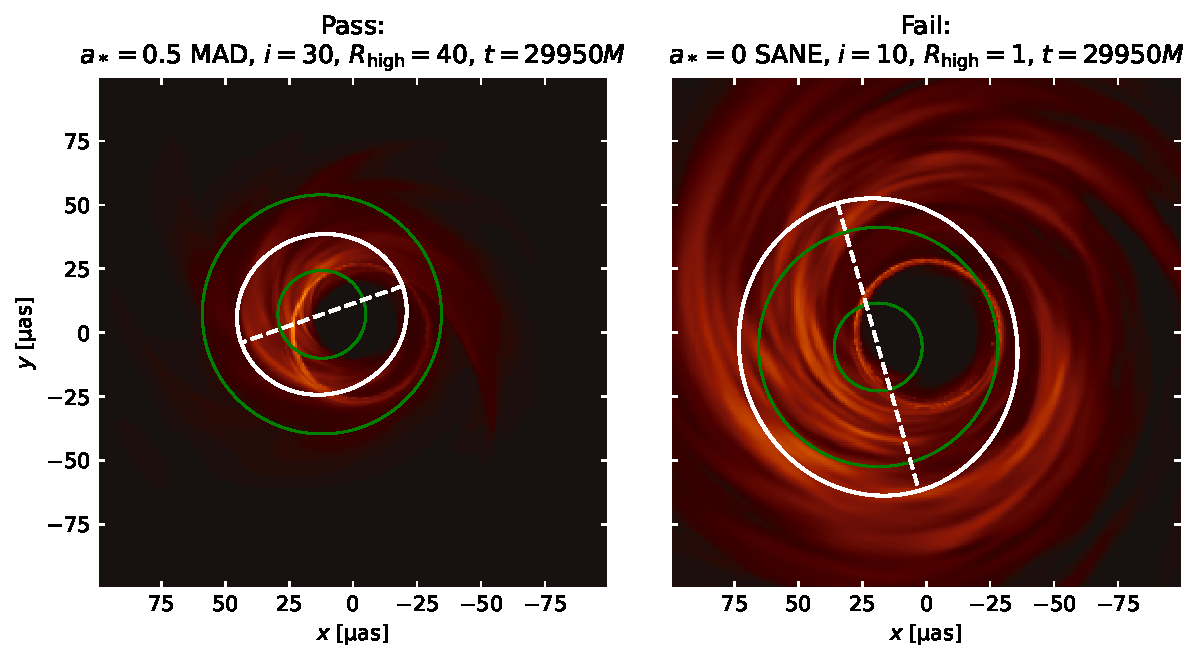
\includegraphics[width=0.75\textwidth]{figures/passfail_sz.pdf}
  \caption{Second moment constraint example.  Left: passing snapshot; right: failing snapshot.  The model is rejected if $< 1\%$ of model snapshots pass. The solid white ellipse  represents the second moments of the image, and the dashed line shows the major axis.  The two green circles show the observed lower and upper limits from \citetalias{PaperIII}. The snapshot is accepted if either the major or minor axis lies between the lower and upper limits.
  }
  \label{fig:passfail_sz}
\end{figure*}

%------------------------------------------------------------------------------
\subsubsection{EHT Structural Variability}

Fluctuations in the spatial structure of the source will produce fluctuations in VA.  Here we compare  the power spectrum of small-scale structural variability from EHT observations with the predictions of GRMHD models.

A nonparametric technique to measure the variance of the spatially-detrended VAs at a location in the $(u,v)$-plane is described in \citet{NoiseModeling} and briefly summarized here.  We use EHT observations of \sgra from April 5, 6, 7, and 10 (notice that April 11 was excluded).  To exclude correlations associated with  variations in the total flux we normalize the VA data with the contemporaneous intrasite lightcurve \citep{Georgiev_2022}.  The lightcurve-normalized visibility amplitudes are then linearly detrended, and variances are computed and azimuthally averaged \citep{NoiseModeling}.  The result, $\sigma_\text{var}^2 (|u|)$, is a measure of the fractional structural variability as a function of baseline length $|u|$.  The $\sigma_\text{var}^2 (|u|)$ is included in an inflated error budget when making images of and fitting models to the 2017 EHT observations of \sgra \citepalias{PaperIII, PaperIV}.

This quantity can be measured from the GRMHD simulations; see \citet{Georgiev_2022}. For all simulations reported here $\sigma_\text{var}^2$ is well-approximated by a broken power law with parameters that are nearly universal among simulations.
% cfg rewrite
The $\sigma_\text{var}^2$ is measured over a four-day period, which is longer than the typical duration of our models.  We therefore expect that model values will be biased downward compared to the data.  We control for this using multiple simulations with the same parameters and by subdividing the analysis of long simulations into windows.
The uncertainties in the measurement from the GRMHD simulations due to simulation resolution, the fast-light approximation, and code differences are small compared to the uncertainty due to the variability of $\sigma_\text{var}^2$ due to short simulations \citep{Georgiev_2022}.

The procedure for estimating $\sigma_\text{var}^2 (|u|)$ has been validated using mock datasets generated from a variety of different models.  In particular, it has been tested using the 100 GRMHD models that comprise the calibration and validation sets in \citetalias{PaperIV}, which incorporate all known systematic effects.  Due to sparse $(u,v)$ coverage, short-timescale temporal correlations induce known biases in the recovered variability measurements, requiring an additional $|u|$-dependent calibration prior to direct comparison; this calibration function and its construction are described in \citealt{NoiseModeling}.  The true $\sigma_\text{var}^2 (|u|)$ can be accurately recovered for $2~{\rm G}\lambda\lesssim|u|\lesssim6~{\rm G}\lambda$, limited by ancillary calibration procedures below $2~{\rm G}\lambda$ and statistical uncertainties above $6~{\rm G}\lambda$.  \citetalias{PaperIV} applies this technique to the 2017 EHT observations of \sgra and provides a measurement of a debiased $\sigma_\text{var}^2$.

The measured $\sigma_\text{var}^2$ is well characterized by a power law for $2~{\rm G}\lambda < |u| < 6~{\rm G}\lambda$ \citep{Georgiev_2022}.  For comparison with the models presented here, we distill the $\sigma_{\text{var}}^2$ to two numbers: a normalization at $4~{\rm G}\lambda$, characterized by the amplitude $\afour^2$ and a power law index $b$.  Because the normalization is done in the center of the fit range the estimated $\afour^2=3.7\pm0.8$ and $b=2.5\pm1$ are essentially uncorrelated.

Model predictions for $\afour^2$ and $b$ are computed using the power spectral densities from \citet{Georgiev_2022}.\footnote{\citet{Georgiev_2022} gives the power spectral density of the complex visibility, $\langle\hat{P}(|u|)\rangle$, rather than the VA, and thus $\sigma_\text{var}^2=\langle \hat{P}\rangle/2$. } The anisotropic diffractive scattering kernel from \citet{Johnson_2018} is applied to $\sigma_\text{var}^2(|u|)$ and averaged over relative orientations of the major axis of the scattering kernel and the black hole spin.  These estimates are then azimuthally averaged, and the parameters $\afour^2$ and $b$ are determined from a least-squares linear fit to $\sigma_\text{var}^2(|u|)$ in $2~{\rm G}\lambda < |u| < 6~{\rm G}\lambda$.
